% Provenance (never printed): see sources/outline_sources.md (Year 1: the general
% circulation of the atmosphere, Hadley, Ferrel and polar cells, the ITCZ, Walker cells,
% jet streams, the geostrophic wind, depressions and anticyclones). Exercise and problem
% values in the Book 3 scratch calculator calc/ch28.py; figures from
% figdata/bachelor-1/angular_momentum_wind.py, weather_map.py (an invented map) and
% general_circulation.py (NCEP-NCAR Reanalysis 1, long-term means 1991-2020, datasets
% bachelor-1-ncep-{uwnd-p,vwnd-p,uwnd-sfc,slp,prate-monthly}).
% Physics owns the Coriolis force and the hydrostatic relation (recalled). Book 1 (g8) gave
% the global winds, the convection cell, depressions and anticyclones, isobars and the
% rotation of the wind around them, in words: re-founded here with forces and data.
% ENSO and the monsoons are the Year 2 volume's; the thermal wind the Year 3 volume's.
\chapter{大气环流}\label{ch:b1:atmospheric-circulation}

从欧洲和非洲驶往美洲的帆船，依靠的是
\omterm{def:b1:atmospheric-circulation:winds}{信风}，即热带的稳定东风。更靠近赤道、约 5 度以内，
同样的风减弱消失，位于无风且多持续阵雨的地带，
水手们称之为“无风带”。远在两者之上，约 9 千米
高处，称为\omterm{def:b1:atmospheric-circulation:jet}{急流}的狭窄气流，风速可超过
\qty{440}{km/h}。本章阐释这三者：为何在旋转行星上运动的空气
最终沿等压线而非横穿等压线流动，热带的盈余如何在赤道两侧各驱动一个
巨大的翻转环流圈，
以及离开赤道高空的空气为何转变为西风\omterm{def:b1:atmospheric-circulation:jet}{急流}。
% ledger: nos:trade-winds, nos:doldrums, noaajs:jet

\begin{omfigure}
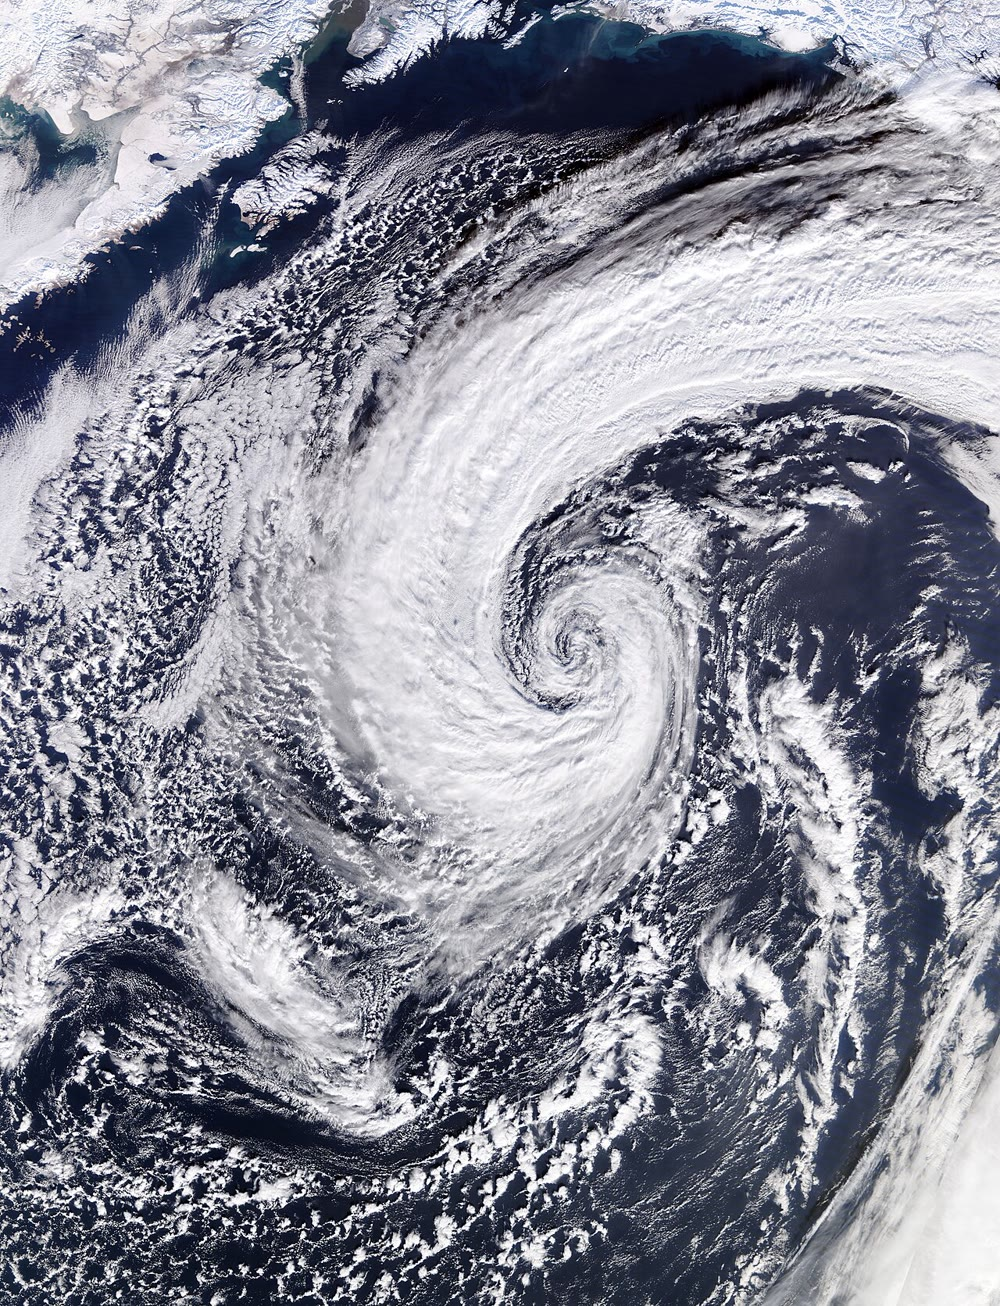
\includegraphics[width=0.5\linewidth]{images/book3/b1-alaska-low.jpg}

{\small 2018 年 1 月 28 日阿拉斯加湾上空的温带\omterm{def:b1:atmospheric-circulation:cyclone}{气旋}，由轨道上的 MODIS 仪器所见；
阿拉斯加被雪覆盖的海岸位于左上方，
大致北向朝上。云带逆时针盘旋汇入
中心，北半球低压中的空气即是如此运动。（NASA，MODIS/LANCE，
公有领域，经由维基共享资源。）}
\label{fig:b1:atmospheric-circulation:alaska}
\end{omfigure}
% ledger: commons:alaska-low, nws:cyclone

\begin{recall}
物理学各册给出了静力平衡关系与科里奥利力：在
角速度为 $\vec\Omega$ 旋转的参考系中，质量为 $m$ 的物体
相对该参考系以速度 $\vec v$ 运动时，受到虚构力
$-2m\,\vec\Omega\times\vec v$，与运动方向垂直。对地球而言，
$\Omega = 2\pi/T_\star$，其中恒星日 $T_\star = \qty{23.9345}{h}$，即
$\Omega = \qty{7.292e-5}{rad.s^{-1}}$。第 1 册介绍了全球风系（\omterm{def:b1:atmospheric-circulation:winds}{信风}、
\omterm{def:b1:atmospheric-circulation:winds}{西风带}、极地东风带）、对流环流圈、低压与\omterm{def:b1:atmospheric-circulation:cyclone}{反气旋}、
天气图上的等压线，以及风绕中心的
旋转。\Cref{ch:b1:fluid-envelopes-structure}给出了\omterm{def:b1:fluid-envelopes-structure:standard-atmosphere}{标准大气}与
\omterm{def:b1:fluid-envelopes-structure:lapse-rate}{干绝热递减率}，\cref{ch:b1:radiation-heat-transport}给出了环流
所输送的向极热量。
% ledger: earth:Trot, nws:coriolis
\end{recall}

\section{运动空气所受的力}\label{sec:b1:atmospheric-circulation:forces}

一团空气受到周围空气压强的推动、
受重力牵引，近地面受摩擦力减慢，从旋转的地球上看，还受科里奥利力的偏转。
重力与竖直方向的压强力几乎精确平衡，
这就是静力平衡关系。天气由
水平方向上剩余的力所决定。

\begin{definition}[气压梯度力]\label{def:b1:atmospheric-circulation:pgf}
称\emph{气压梯度力}\index{气压梯度力}为周围流体的压强作用于
流体微团上的净力。单位质量上的
力为 $-(1/\rho)\nabla p$，其中 $\rho$ 为密度，$\nabla p$ 为压强梯度，
方向由高压指向低压，即垂直穿过等压线。
\end{definition}
% ledger: nws:geostrophic

\begin{proposition}[气压梯度力]\label{prop:b1:atmospheric-circulation:pgf}
对体积为 $\mathrm dV$、密度为 $\rho$ 的流体微团，周围流体的压强
施加的力为 $-\nabla p\,\mathrm dV$，对应加速度
$-(1/\rho)\nabla p$。
\end{proposition}

\begin{proof}
取一个棱沿坐标轴方向、棱长分别为
$\mathrm dx$、$\mathrm dy$、$\mathrm dz$ 的小方盒。在 $x$ 处的面上，压强沿 $+x$ 方向施力
大小为 $p(x)\,\mathrm dy\,\mathrm dz$；在 $x + \mathrm dx$ 处的面上，沿 $-x$ 方向
施力，大小为 $p(x + \mathrm dx)\,\mathrm dy\,\mathrm dz$。沿
$x$ 方向的合力为 $[p(x) - p(x + \mathrm dx)]\,\mathrm dy\,\mathrm dz = -(\partial p/\partial
x)\,\mathrm dV$，沿 $y$、$z$ 方向同理。总力为 $-\nabla p\,
\mathrm dV$；除以质量 $\rho\,\mathrm dV$ 即得加速度。
\end{proof}

均匀的压强不产生合力，只有压强的差异才推动空气。天气图上，
水平梯度由等压线读出：其大小为相邻两条等压线之间的压强差
除以它们之间的距离。若两条等压线相差 \qty{4}{hPa}，
相距 \qty{400}{km}，海平面处 $\rho \approx \qty{1.225}{kg.m^{-3}}$，
则加速度为 $400/(1.225 \times \num{4e5}) = \qty{8.2e-4}{m.s^{-2}}$，小于 $g$ 的万分之一，
却足以使静止的空气在
三个半小时内达到 \qty{10}{m/s}。
% ledger: ussa76:sea-level

空气所受的科里奥利力，源于人们在旋转的地球上观测它。其
水平分量仅通过一个数随\omterm{def:b1:spherical-astronomy:geographic}{纬度}变化。

\begin{definition}[科里奥利参数]\label{def:b1:atmospheric-circulation:coriolis-parameter}
\omterm{def:b1:spherical-astronomy:geographic}{纬度} $\varphi$ 处的\emph{科里奥利参数}\index{科里奥利参数}为
$f = 2\Omega\sin\varphi$，其中 $\Omega$ 为地球的角速度。它
在北半球为正，南半球为负，赤道处为零，
在两极最大，$2\Omega = \qty{1.458e-4}{s^{-1}}$。
\end{definition}
% ledger: earth:Trot

\begin{proposition}[水平科里奥利加速度]\label{prop:b1:atmospheric-circulation:coriolis}
设水平风 $\vec v$ 位于\omterm{def:b1:spherical-astronomy:geographic}{纬度} $\varphi$ 处，
则科里奥利加速度的水平分量为 $-f\,\vec k\times\vec v$，其中 $\vec k$ 为竖直向上的
单位矢量：其大小为 $|f|\,|\vec v|$，方向与风向垂直，
北半球指向风的右侧，南半球指向左侧。
\end{proposition}

\begin{proof}
取局地坐标轴，$x$ 指向东，$y$ 指向北，$z$ 指向上。地球自转矢量位于
子午面内，与北方地平线夹角为 $\varphi$：$\vec\Omega =
\Omega(0, \cos\varphi, \sin\varphi)$。对 $\vec v = (u, v, 0)$，
\[
  \vec\Omega\times\vec v = \Omega\,(-v\sin\varphi,\ u\sin\varphi,\ -u\cos\varphi),
  \qquad -2\vec\Omega\times\vec v = (f v,\ -f u,\ 2\Omega u\cos\varphi).
\]
由于 $\vec k\times\vec v = (-v, u, 0)$，水平分量 $(fv, -fu)$ 即为
$-f\,\vec k\times\vec v$。矢量 $\vec k\times\vec v$ 为 $\vec v$ 俯视时
逆时针旋转 \ang{90} 所得；其反向即 $\vec v$ 顺时针旋转，
在 $f > 0$ 时指向右侧，$f < 0$ 时指向左侧。
\end{proof}
% ledger: earth:Trot

竖直分量 $2\Omega u\cos\varphi$ 至多为 \qty{1.5e-3}{m.s^{-2}}，
对应风速 \qty{10}{m/s}，约为 $g$ 的 \num{1.5e-4} 倍，静力平衡
可将其吸收。水平分量虽小，
但在摩擦层以上的自由大气中无可匹敌，数小时之内便塑造每一股风。

近地面处，空气也与地表相摩擦。在最低的一千米内，即气象学家所称的
摩擦层，摩擦力既改变风速，
也改变风向；湍流涡旋把地表阻力向上输送，
此力大致与风向相反，并随风速增大而增大。在其上方的自由大气中，
摩擦力很小。
% ledger: nws:friction-layer

\section{地转风}\label{sec:b1:atmospheric-circulation:geostrophic}

\begin{definition}[地转平衡，地转风]\label{def:b1:atmospheric-circulation:geostrophic}
若水平流动的\omterm{def:b1:atmospheric-circulation:pgf}{气压梯度力}与其科里奥利力
相互抵消，则称该流动处于\emph{地转平衡}\index{地转平衡}。\emph{地转
风}\index{地转风} $\vec v_g$ 是在给定
气压场下实现该平衡的风：$-(1/\rho)\nabla p - f\,\vec k\times\vec v_g = \vec 0$。
\end{definition}
% ledger: nws:geostrophic

\begin{theorem}[地转风]\label{thm:b1:atmospheric-circulation:geostrophic}
在远离赤道处，
\[
  \vec v_g = \frac{1}{\rho f}\,\vec k\times\nabla p, \qquad
  |\vec v_g| = \frac{|\nabla p|}{\rho\,|f|} .
\]
\omterm{def:b1:atmospheric-circulation:geostrophic}{地转风}沿等压线吹，等压线越密集处风速越大。
北半球时低压位于其左侧；南半球
则位于其右侧。
\end{theorem}

\begin{proof}
对水平矢量 $\vec w$，有 $\vec k\times(\vec k\times\vec w) = -\vec w$。
以 $\vec k\times$ 作用于平衡式 $f\,\vec k\times\vec v_g = -(1/\rho)\nabla p$ 两边，
得 $-f\vec v_g = -(1/\rho)\,\vec k\times\nabla p$，由此得上式，
其在 $f \neq 0$ 时成立。由于 $\vec k\times\nabla p$ 与 $\nabla p$ 垂直，风
速与梯度垂直，即沿等压线；其大小为 $|\nabla
p|/(\rho|f|)$。矢量 $\vec k\times\nabla p$ 为梯度
逆时针旋转 \ang{90} 所得。面向其方向时，指向高压的梯度
位于右侧，因此低压位于左侧；$f > 0$ 时，风向
与 $\vec k\times\nabla p$ 同向，$f < 0$ 时则为其反向。
\end{proof}

\begin{example}[由等压线读出的风]\label{ex:b1:atmospheric-circulation:geostrophic}
北纬 \ang{50} 处，$f = 2 \times \num{7.292e-5} \times \sin\ang{50} = \qty{1.117e-4}{s^{-1}}$。
两等压线相隔 \qty{4}{hPa}，距离为 \qty{400}{km}，于是 $|\nabla p| = 400/\num{4e5} =
\qty{1.0e-3}{Pa.m^{-1}}$。取 $\rho = \qty{1.225}{kg.m^{-3}}$，\omterm{def:b1:atmospheric-circulation:geostrophic}{地转风}
为 $\num{1.0e-3}/(1.225 \times \num{1.117e-4}) = \qty{7.3}{m/s}$。相同间距在
北纬 \ang{20} 处，
$f$ 不足前者的一半，将给出 \qty{16.4}{m/s}。
\end{example}
% ledger: earth:Trot, ussa76:sea-level

平衡并非瞬时建立。气压梯度推动的空气，在科里奥利力作用下
以速率 $f$ 偏转，每 $2\pi/f$ 时间约转过一周，
北纬 \ang{50} 处约为十六小时；持续数小时以上、尺度大于
数百千米的系统接近\omterm{def:b1:atmospheric-circulation:geostrophic}{地转平衡}。赤道附近 $f$ 趋于
零，公式失效，深热带的风
并非\omterm{def:b1:atmospheric-circulation:geostrophic}{地转风}。

\begin{omfigure}
\begin{tikzpicture}[>={Stealth[length=2.2mm]}, font=\scriptsize]
  % left panel: geostrophic balance
  \begin{scope}
    \draw[isobar] (-2.4,1.2) -- (2.4,1.2) node[right] {\qty{996}{hPa}};
    \draw[isobar] (-2.4,0) -- (2.4,0) node[right] {\qty{1000}{hPa}};
    \draw[isobar] (-2.4,-1.2) -- (2.4,-1.2) node[right] {\qty{1004}{hPa}};
    \node[pressure low] at (0,2.0) {L};
    \node[pressure high] at (0,-2.0) {H};
    \fill (0,0) circle (1.6pt);
    \draw[->, very thick, omThm] (0,0) -- (0,1.0);
    \node[omThm, anchor=east] at (-0.08,0.6) {气压梯度};
    \draw[->, very thick, omDef] (0,0) -- (0,-1.0);
    \node[omDef, anchor=east] at (-0.08,-0.6) {科里奥利力};
    \draw[->, line width=1.6pt, black] (0,0) -- (1.9,0) node[above, pos=0.75] {风 $\vec v_g$};
    \node[anchor=north] at (0,-2.4) {无摩擦：地转};
  \end{scope}
  % right panel: with friction (alpha = 25 deg, V = Vg cos alpha)
  \begin{scope}[xshift=7.4cm]
    \draw[isobar] (-2.4,1.2) -- (2.4,1.2) node[right] {\qty{996}{hPa}};
    \draw[isobar] (-2.4,0) -- (2.4,0) node[right] {\qty{1000}{hPa}};
    \draw[isobar] (-2.4,-1.2) -- (2.4,-1.2) node[right] {\qty{1004}{hPa}};
    \node[pressure low] at (0,2.0) {L};
    \node[pressure high] at (0,-2.0) {H};
    \fill (0,0) circle (1.6pt);
    \draw[->, very thick, omThm] (0,0) -- (0,1.0);
    \node[omThm, anchor=east] at (-0.08,0.6) {气压梯度};
    \draw[->, very thick, omDef] (0,0) -- ({1.0*cos(25)*sin(25)},{-1.0*cos(25)*cos(25)});
    \node[omDef, anchor=west] at (0.42,-0.62) {科里奥利力};
    \draw[->, very thick, omMeth] (0,0) -- ({-1.0*sin(25)*cos(25)},{-1.0*sin(25)*sin(25)})
      node[below left, inner sep=1pt] {摩擦力};
    \draw[->, line width=1.6pt, black] (0,0) -- ({1.9*cos(25)*cos(25)},{1.9*cos(25)*sin(25)})
      node[above, inner sep=2pt] {风 $\vec v$};
    \draw[black!50, dashed] (0,0) -- (1.9,0);
    \draw[black!60] (1.0,0) arc[start angle=0, end angle=25, radius=1.0];
    \node[black!70] at (1.22,0.22) {$\alpha$};
    \node[anchor=north] at (0,-2.4) {有摩擦：减速，斜穿等压线};
  \end{scope}
\end{tikzpicture}

{\small 北半球空气团所受的力，北侧为低压。
左图：自由大气中，\omterm{def:b1:atmospheric-circulation:pgf}{气压梯度力}（红色）与
科里奥利力（蓝色）相互抵消，风沿等压线吹，低压位于其左侧。
右图：近地面处，摩擦力（绿色）与风向相反；三力
平衡的条件是风速变小，并偏转角度 $\alpha$，
朝向低压一侧（图中取 $\alpha = \ang{25}$，阻力取
\cref{prop:b1:atmospheric-circulation:friction}）。}
\label{fig:b1:atmospheric-circulation:balance}
\end{omfigure}

\begin{proposition}[摩擦使风转向低压]\label{prop:b1:atmospheric-circulation:friction}
设定常水平风 $\vec v$ 受\omterm{def:b1:atmospheric-circulation:pgf}{气压梯度力}、
科里奥利力及摩擦力 $-\vec v/\tau$ 作用，其中 $\tau > 0$，位于
\omterm{def:b1:spherical-astronomy:geographic}{纬度} $f > 0$ 处。则风指向低压穿过等压线，
其夹角为 $\alpha$，$\tan\alpha = 1/(f\tau)$，速率为 $|\vec v| =
|\vec v_g|\cos\alpha$，小于\omterm{def:b1:atmospheric-circulation:geostrophic}{地转风}。
\end{proposition}

\begin{proof}
设 $V = |\vec v|$，$\hat v$ 为沿风向的单位矢量，$\hat n$ 为
与之垂直、位于其左侧的单位矢量。平衡式为 $-(1/\rho)\nabla p - f\,
\vec k\times\vec v - \vec v/\tau = \vec 0$，且 $\vec k\times\vec v = V\hat n$。
沿 $\hat v$ 方向：$-(1/\rho)\,\nabla p\cdot\hat v = V/\tau > 0$，故风具有一个
分量沿气压梯度向下，即指向低压。沿 $\hat n$ 方向：
$-(1/\rho)\,\nabla p\cdot\hat n = fV$。\omterm{def:b1:atmospheric-circulation:pgf}{气压梯度力}大小为 $P =
|\nabla p|/\rho = f|\vec v_g|$，因此其沿风向的分量为 $V/\tau$，
垂直于风向的分量为 $fV$：它与风向成角 $\beta$，$\tan\beta =
1/(f\tau)$，且 $P^2 = V^2(f^2 + 1/\tau^2)$。等压线与气压梯度
垂直，故风穿过等压线的角度为 $\alpha = \beta$，且 $V = P/\sqrt{f^2 +
1/\tau^2} = (P/f)\cos\alpha = |\vec v_g|\cos\alpha$。
\end{proof}

地表越粗糙，阻力越大，$\tau$ 越短，偏转角越大：
风穿过等压线的角度在陆地上比在海上更陡。实际摩擦力
与风速并非严格线性关系，但结论——风速变小，并偏向
低压一侧——具有普遍性。

\begin{remark}[梯度风]\label{rem:b1:atmospheric-circulation:gradient}
在一个中心周围，等压线呈弯曲状，沿其运动的空气受到指向
曲率中心的加速度 $V^2/r$（对半径为 $r$ 的圆周）。在北半球低压周围，
\omterm{def:b1:atmospheric-circulation:pgf}{气压梯度力}必须大于
科里奥利力：$fV + V^2/r = f|\vec v_g|$，此风称为梯度风，
其强度弱于\omterm{def:b1:atmospheric-circulation:geostrophic}{地转风}。在高压周围，科里奥利力必须大于
\omterm{def:b1:atmospheric-circulation:pgf}{气压梯度力}，即 $fV - V^2/r = f|\vec v_g|$：风更强，但
方程有解的条件是 $|\vec v_g| \leq fr/4$，此条件排除了\omterm{def:b1:atmospheric-circulation:cyclone}{反气旋}中心附近的强
气压梯度（见\cref{exo:b1:atmospheric-circulation:10}）。
\end{remark}

\section{低压与反气旋}\label{sec:b1:atmospheric-circulation:cyclones}

\begin{definition}[气旋、反气旋]\label{def:b1:atmospheric-circulation:cyclone}
称\emph{气旋}\index{气旋}为围绕一个
低压中心的大尺度风环流，即低压；\emph{反气旋}\index{反气旋}为
围绕一个高压中心的环流。气旋在北半球逆时针旋转，
在南半球顺时针旋转；
反气旋的旋转方向则相反。
\end{definition}
% ledger: nws:cyclone

旋转方向由\cref{thm:b1:atmospheric-circulation:geostrophic}可得：
在北半球，低压位于左侧的风绕低压
呈逆时针方向流动，绕高压则呈顺时针。从太空望去，低压的云系
勾勒出其旋转轨迹（即本章开头的照片）；在
南半球，螺旋形态呈镜像对称。
% ledger: nws:cyclone, commons:alaska-low

\begin{history}[拜斯·巴洛定律，1857 年]
1857 年，荷兰气象学家 C.~H.~D. 拜斯·巴洛提出一条得自
观测的规则：在北半球，背风而立者，左侧为低压，右侧为高压；
在南半球则相反。
他不知道美国气象学家威廉·费雷尔
早已从理论上推出此结论，后来承认了费雷尔的优先权。
\omterm{def:b1:atmospheric-circulation:geostrophic}{地转风}即是以方程表达的这一定律。
\end{history}
% ledger: skybrary:buys-ballot

摩擦又带来一个重要的变化。近地面处，风穿过等压线
指向低压（见\cref{prop:b1:atmospheric-circulation:friction}）：在
低压周围，空气向内螺旋，在近地面辐合，必须上升。上升
空气膨胀降温，降温率为\omterm{def:b1:fluid-envelopes-structure:lapse-rate}{干绝热递减率}
（见\cref{ch:b1:fluid-envelopes-structure}），一旦饱和，其水蒸气
凝结：低压带来云和雨。在\omterm{def:b1:atmospheric-circulation:cyclone}{反气旋}周围，近地面空气
向外螺旋；上方空气下沉以补充，因压缩而增温，且
其云蒸发：\omterm{def:b1:atmospheric-circulation:cyclone}{反气旋}带来稳定、通常晴朗的天气。
% ledger: nws:dalr

下图为一个虚构的例子，系计算而非观测所得：一个低压
深 \qty{28}{hPa}，一个\omterm{def:b1:atmospheric-circulation:cyclone}{反气旋}高 \qty{20}{hPa}，背景气压为
\qty{1013}{hPa}，中心位于北纬 \ang{50} 附近。各测站的风羽
表示依据\cref{thm:b1:atmospheric-circulation:geostrophic}由地图算出的\omterm{def:b1:atmospheric-circulation:geostrophic}{地转风}。

\begin{omfigure}
\pgfplotstableread{figdata/out/bachelor-1-weather_map-stations.dat}\wmstations
\pgfplotstableread{figdata/out/bachelor-1-weather_map-labels.dat}\wmlabels
\begin{tikzpicture}
\begin{axis}[x=0.0038cm, y=0.0038cm, disabledatascaling, anchor=origin,
  xmin=-1800, xmax=1800, ymin=-1200, ymax=1200, xtick=\empty, ytick=\empty,
  axis background/.style={fill=blue!4}, clip=true]
% figdata/bachelor-1/weather_map.py (invented pressure field); ledger: earth:Trot, ussa76:sea-level
\addplot[isobar, unbounded coords=jump] table[x=x, y=y] {figdata/out/bachelor-1-weather_map-isobars.dat};
\addplot[black!45, dashed, domain=-1800:1800] {0};
\addplot[only marks, mark=none, nodes near coords, point meta=explicit symbolic,
  nodes near coords style={font=\tiny, fill=blue!4, inner sep=0.5pt, anchor=center}]
  table[x=x, y=y, meta=p] {\wmlabels};
\node[pressure low] at (axis cs:-500,150) {低};
\node[pressure high] at (axis cs:1050,-250) {高};
\node[font=\tiny, anchor=south west, black!60] at (axis cs:-1790,5) {北纬 \ang{50}};
\end{axis}
\pgfplotstablegetrowsof{\wmstations}
\pgfmathtruncatemacro{\wmlast}{\pgfplotsretval-1}
\begin{scope}
\clip (-6.84,-4.56) rectangle (6.84,4.56);
\foreach \i in {0,...,\wmlast}{
  \pgfplotstablegetelem{\i}{x}\of\wmstations \let\wx\pgfplotsretval
  \pgfplotstablegetelem{\i}{y}\of\wmstations \let\wy\pgfplotsretval
  \pgfplotstablegetelem{\i}{speed_kn}\of\wmstations \let\ws\pgfplotsretval
  \pgfplotstablegetelem{\i}{from_deg}\of\wmstations \let\wd\pgfplotsretval
  \pic[transform shape] at ({\wx*0.0038},{\wy*0.0038}) {windbarb={\ws}{\wd}};
}
\end{scope}
\pic[transform shape] at (-6.5,-4.0) {scalebar={1.9}{\qty{500}{km}}};
\pic[scale=0.7, transform shape] at (-6.45,3.2) {northarrow};
\end{tikzpicture}

{\small 一幅虚构的海平面气压图，位于北纬 \ang{50} 附近（等压线每
\qty{4}{hPa} 一条；中心气压分别为 \qty{986}{hPa} 和 \qty{1033}{hPa}）。每个风羽
指向其所在测站的\omterm{def:b1:atmospheric-circulation:geostrophic}{地转风}，羽杆指向风的来向；全羽为
\qty{10}{kn}，半羽为 \qty{5}{kn}，旗为
\qty{50}{kn}（\qty{1}{kn} = \qty{0.514}{m/s}）。风在低压周围逆时针旋转，
在高压周围顺时针旋转，在两者之间等压线最密集处风最强，
可达 \qty{36}{m/s}。}
\label{fig:b1:atmospheric-circulation:weather-map}
\end{omfigure}
% ledger: earth:Trot, ussa76:sea-level (computed in figdata/bachelor-1/weather_map.py)

\section{三圈环流}\label{sec:b1:atmospheric-circulation:cells}

全球平均并经多年平均后，南北向吹的风较弱，
至多每秒几米，但它们输送大量空气。其格局
最好从赤道与两极之间流动的气团来看。

\begin{definition}[平均经向流函数]\label{def:b1:atmospheric-circulation:streamfunction}
\emph{平均经向流函数}\index{平均经向流函数}
$\psi(p, \varphi)$ 是每秒向北穿过\omterm{def:b1:spherical-astronomy:geographic}{纬度}
$\varphi$ 处、位于气压面 $p$ 以上的空气质量，取纬向与时间平均：
\[
  \psi(p, \varphi) = \frac{2\pi a_\oplus\cos\varphi}{g}\int_0^p [v]\,\mathrm dp' ,
\]
其中 $[v]$ 为绕纬线平均的北向风。它的单位为
\unit{kg.s^{-1}}。
\end{definition}

由静力关系 $\mathrm dp' = -\rho g\,\mathrm dz$，$2\pi a_\oplus
\cos\varphi\,[v]\,\mathrm dp'/g$ 为穿过纬线圈的质量通量。
在 $p$ 以上穿过纬线的空气，必在 $p$ 以下以相反方向穿过它，
因为质量不会堆积：$\psi$ 在地面和顶部均为零，其等值线
即为平均环流的路径。当 $\psi > 0$ 时，若北极位于右侧，此环流圈顺时针转动，
即上层向北、下层向南。

\begin{omfigure}
\begin{tikzpicture}
\begin{groupplot}[group style={group size=1 by 2, vertical sep=1.3cm},
  width=0.82\linewidth, height=4.6cm, view={0}{90}, xmin=-70, xmax=70, ymin=100,
  ymax=1000, y dir=reverse, ytick={200,400,600,800,1000}, xtick={-60,-40,...,60},
  tick label style={font=\scriptsize}, label style={font=\small},
  ylabel={气压 (\unit{hPa})},
  colormap={omdiv}{rgb255=(33,102,172) rgb255=(146,197,222) rgb255=(247,247,247)
    rgb255=(244,165,130) rgb255=(178,24,43)},
  point meta min=-22, point meta max=22, colorbar,
  colorbar style={width=0.25cm, y dir=normal, ytick={-20,-10,0,10,20}, tick label style={font=\scriptsize},
    ylabel={$\psi$ (\qty{e10}{kg.s^{-1}})}, ylabel style={font=\scriptsize}},
  axis on top, grid=none]
\nextgroupplot[title={12 月至次年 2 月}, title style={font=\small}]
% figdata/bachelor-1/general_circulation.py; ledger: data:b3-ncep-circ, psl:ncep-r1
\addplot3[surf, shader=interp, mesh/ordering=x varies, mesh/cols=73]
  table[x=lat, y=p, z=psi] {figdata/out/bachelor-1-general_circulation-psi-djf.dat};
\addplot3[black, line width=0.5pt, unbounded coords=jump]
  table[x=lat, y=p, z expr=40] {figdata/out/bachelor-1-general_circulation-psi0-djf.dat};
\nextgroupplot[title={6--8 月}, title style={font=\small}, xlabel={纬度 (\unit{\degree})}]
\addplot3[surf, shader=interp, mesh/ordering=x varies, mesh/cols=73]
  table[x=lat, y=p, z=psi] {figdata/out/bachelor-1-general_circulation-psi-jja.dat};
\addplot3[black, line width=0.5pt, unbounded coords=jump]
  table[x=lat, y=p, z expr=40] {figdata/out/bachelor-1-general_circulation-psi0-jja.dat};
\end{groupplot}
\end{tikzpicture}

{\small 北半球冬季（上）与北半球夏季（下）的\omterm{def:b1:atmospheric-circulation:streamfunction}{平均经向流函数}，
取自 NCEP-NCAR Reanalysis~1 的纬向平均北向风，平均期为 1991--2020 年
（数据由 NOAA PSL 提供）。红色：此视图中为顺时针环流圈（其南侧上升），
蓝色：逆时针；黑色：分隔各环流圈的零线。
冬季\omterm{def:b1:atmospheric-circulation:cells}{哈得来环流圈}跨越赤道，
远大于夏季者。}
\label{fig:b1:atmospheric-circulation:psi}
\end{omfigure}
% ledger: data:b3-ncep-circ, psl:ncep-r1 (computed in figdata/bachelor-1/general_circulation.py)

年平均意义上，再分析资料显示赤道两侧有两个较强的环流圈，
其极大值约为 \qty{8.7e10}{kg/s}，分别位于北纬 \ang{15} 和南纬 \ang{15} 附近（在 \qty{400}{hPa} 处）；
在 \qty{500}{hPa} 处，其向极边缘分别位于北纬 \ang{33} 和南纬 \ang{32}。
在它们的极向一侧，另有两个较弱的环流圈转向相反，分别延伸至北纬约 \ang{61} 和南纬约 \ang{64}。
季节使图景发生变化：12 月至次年 2 月，即北半球冬季，
在赤道以南上升、在北半球副热带下沉的环流圈，其强度为
\qty{21.4e10}{kg/s}，范围从南纬 \ang{13} 延伸至北纬 \ang{31}；6--8 月，
其镜像环流的强度为 \qty{18.9e10}{kg/s}，范围从北纬 \ang{17} 延伸至南纬 \ang{29}。
% ledger: data:b3-ncep-circ (computed in figdata/bachelor-1/general_circulation.py)

\begin{definition}[哈得来环流圈、费雷尔环流圈和极地环流圈；副热带高压]\label{def:b1:atmospheric-circulation:cells}
每个半球的平均经向环流有三个环流圈。\emph{哈得来
环流圈}\index{哈得来环流圈}在赤道附近上升，高层流向极地，
在约 \ang{30} 处下沉，并在地面回流至赤道。\emph{费雷尔
环流圈}\index{费雷尔环流圈}位于约 \ang{30} 与 \ang{60} 之间，转向相反：
在约 \ang{30} 处下沉，在约 \ang{60} 处上升，其地面气流指向极地。\emph{极地
环流圈}\index{极地环流圈}最小、最弱，在约 \ang{60} 处上升，
在极点上空下沉，并在地面回流至约 \ang{60}。
\emph{副热带高压}\index{副热带高压}是高海平面气压带，
位于北纬与南纬约 \ang{30} 附近，处于哈得来环流圈的下沉支之下。
\end{definition}
% ledger: noaajs:cells, nws:ferrel-cell, nws:winds

\begin{definition}[信风、西风带]\label{def:b1:atmospheric-circulation:winds}
\emph{信风}\index{信风}是持续吹拂的地面风，
由\omterm{def:b1:atmospheric-circulation:cells}{副热带高压}吹向赤道低压，受科里奥利力作用，
在北半球转为东北风，在南半球
转为东南风。\emph{西风带}\index{西风带}是中\omterm{def:b1:spherical-astronomy:geographic}{纬度}盛行的西风，
位于约 \ang{35} 至 \ang{60} 之间。其极向一侧盛行的是
极地东风带。
\end{definition}
% ledger: nws:winds, noaajs:cells

各环流圈的地面分支解释了其风。\omterm{def:b1:atmospheric-circulation:cells}{哈得来环流圈}的回流
流向赤道，受科里奥利力作用向西偏转：即
\omterm{def:b1:atmospheric-circulation:winds}{信风}。\omterm{def:b1:atmospheric-circulation:cells}{费雷尔环流圈}的地面气流指向极地，并受科里奥利力向东偏转：
即\omterm{def:b1:atmospheric-circulation:winds}{西风带}。在再分析资料的年平均中，地面以上的纬向风
在北纬 \ang{15} 为 \qty{-3.5}{m/s}，在南纬 \ang{15} 为 \qty{-4.4}{m/s}（负值
表示来自东方），在北纬 \ang{45} 为 \qty{+1.9}{m/s}，在南纬 \ang{45} 为 \qty{+6.5}{m/s}；
海平面气压在北纬约 \ang{35} 处达到峰值 \qty{1017.5}{hPa}，并在南纬约 \ang{32} 处
为 \qty{1018.7}{hPa}，并在南纬 \ang{60} 处降至 \qty{988}{hPa}，即
南大洋的深槽。
% ledger: data:b3-ncep-circ (computed in figdata/bachelor-1/general_circulation.py)

\begin{omfigure}
\begin{tikzpicture}[>={Stealth[length=1.8mm]}, font=\scriptsize]
  % left: the globe with the surface winds
  \def\R{2.6}
  \fill[blue!7] (0,0) circle (\R);
  \draw (0,0) circle (\R);
  \foreach \l in {-60,-30,30,60} {
    \pgfmathsetmacro{\y}{\R*sin(\l)}\pgfmathsetmacro{\x}{\R*cos(\l)}
    \draw[black!45, dashed] (-\x,\y) -- (\x,\y);}
  \draw[black!60] (-\R,0) -- (\R,0);
  \foreach \s in {1,-1} {
    \foreach \x in {-1.7,-0.7,0.3} {
      \draw[->, omThm, line width=0.9pt] (\x+0.3,\s*0.95) -- (\x-0.3,\s*0.45);}
    \foreach \x in {-1.0,0.2} {
      \draw[->, omDef, line width=0.9pt] (\x-0.3,\s*1.45) -- (\x+0.3,\s*1.9);}
    \draw[->, omMeth, line width=0.9pt] (0.25,\s*2.45) -- (-0.25,\s*2.2);
  }
  \node[fill=blue!7, inner sep=1pt, anchor=west] at (0.95,0.72) {东北信风};
  \node[fill=blue!7, inner sep=1pt, anchor=west] at (0.95,-0.72) {东南信风};
  \node[fill=blue!7, inner sep=1pt, anchor=west] at (0.55,1.72) {西风带};
  \node[fill=blue!7, inner sep=1pt, anchor=west] at (0.55,-1.72) {西风带};
  \node[anchor=south] at (0,\R+0.02) {极地东风带};
  \node[anchor=north] at (0,-\R-0.02) {极地东风带};
  \node[anchor=east, align=right] at (-\R-0.05,0) {赤道低压 \\(ITCZ)};
  \node[anchor=east, align=right] at ({-\R*cos(30)-0.05},{\R*sin(30)}) {副热带高压};
  \node[anchor=east, align=right] at ({-\R*cos(30)-0.05},{-\R*sin(30)}) {副热带高压};
  \node[anchor=east] at ({-\R*cos(60)-0.05},{\R*sin(60)}) {副极地低压};
  \node[anchor=east] at ({-\R*cos(60)-0.05},{-\R*sin(60)}) {副极地低压};
  % right: meridional section of the Northern Hemisphere
  \begin{scope}[xshift=4.3cm, yshift=-1.4cm]
    \draw[->] (0,0) -- (6.3,0);
    \foreach \l/\t in {0/\ang{0},2/北纬 \ang{30},4/北纬 \ang{60},6/北纬 \ang{90}}
      \draw (\l,0.06) -- (\l,-0.06) node[below] {\t};
    \draw[black!45, dashed] (0,2.6) .. controls (2.4,2.6) and (2.8,1.9) .. (6,1.7)
      node[above left, black!60] {对流层顶};
    \def\cellcw#1#2#3#4{\draw[line width=0.9pt, omThm, postaction=decorate,
      decoration={markings, mark=at position 0.25 with {\arrow{Stealth[length=2mm]}},
      mark=at position 0.75 with {\arrow{Stealth[length=2mm]}}}]
      (#1+#3,#2) arc[start angle=0, end angle=-360, x radius=#3, y radius=#4];}
    \def\cellccw#1#2#3#4{\draw[line width=0.9pt, omDef, postaction=decorate,
      decoration={markings, mark=at position 0.25 with {\arrow{Stealth[length=2mm]}},
      mark=at position 0.75 with {\arrow{Stealth[length=2mm]}}}]
      (#1+#3,#2) arc[start angle=0, end angle=360, x radius=#3, y radius=#4];}
    \cellcw{1}{1.25}{0.85}{1.05}
    \cellccw{3}{1.0}{0.85}{0.75}
    \cellcw{5}{0.85}{0.85}{0.6}
    \node at (1,1.25) {哈得来};
    \node at (3,1.0) {费雷尔};
    \node at (5,0.85) {极地};
  \end{scope}
\end{tikzpicture}

{\small 左：三圈环流的地面风，位于各气压带之间，
在北半球偏向其运动方向的右侧，在南半球偏向左侧。
右：北半球三个环流圈的经向剖面
（高度未按比例绘制）；南半球与之呈镜像对称。
\omterm{def:b1:atmospheric-circulation:winds}{信风}是\omterm{def:b1:atmospheric-circulation:cells}{哈得来环流圈}的回流支，
\omterm{def:b1:atmospheric-circulation:winds}{西风带}是\omterm{def:b1:atmospheric-circulation:cells}{费雷尔环流圈}的地面支。}
\label{fig:b1:atmospheric-circulation:three-cells}
\end{omfigure}
% ledger: noaajs:cells, nws:winds, nws:ferrel-cell

\begin{history}[哈得来 1735，费雷尔 1856]
1735 年，乔治·哈得来在\emph{Philosophical Transactions}上发表了一篇短文，
探讨一般\omterm{def:b1:atmospheric-circulation:winds}{信风}的成因。为解释\omterm{def:b1:atmospheric-circulation:winds}{信风}，他提出每个半球内存在一个单一环流，
从赤道延伸至极地。
1856 年，威廉·费雷尔出版了\emph{An essay on the winds and currents of the
ocean}，其中指出中\omterm{def:b1:spherical-astronomy:geographic}{纬度}空气在近地面流向极地并向东偏转：
这是对 \ang{35} 至 \ang{60} 之间\omterm{def:b1:atmospheric-circulation:winds}{西风带}的最早描述。
他的论文未给出数学论证；他所描述的环流正是
以其名字命名的那一环流圈。
\end{history}
% ledger: hadley:1735, noaajs:cells, mactutor:ferrel

为何\omterm{def:b1:atmospheric-circulation:cells}{哈得来环流圈}会止于 \ang{30} 附近，
而不像哈得来所设想的那样直达极地？答案在于空气
绕地轴所携带的角动量。

\begin{proposition}[角动量风]\label{prop:b1:atmospheric-circulation:angular-momentum}
\omterm{def:b1:spherical-astronomy:geographic}{纬度}为 $\varphi$ 的一圈空气，相对于地面具有向东风速 $u$，
其关于地轴的绝对角动量（单位质量）为 $M =
(\Omega a_\oplus\cos\varphi + u)\,a_\oplus\cos\varphi$。若静止于\omterm{def:b1:spherical-astronomy:geographic}{纬度} $\varphi_0$ 的一圈空气
在无力矩作用下移动到 $\varphi$，
则其风速为
\[
  u(\varphi) = \Omega a_\oplus\,\frac{\cos^2\varphi_0 - \cos^2\varphi}{\cos\varphi},
  \qquad\text{且自赤道出发时}\qquad
  u(\varphi) = \Omega a_\oplus\,\frac{\sin^2\varphi}{\cos\varphi} .
\]
\end{proposition}

\begin{proof}
\omterm{def:b1:spherical-astronomy:geographic}{纬度}为 $\varphi$ 的一圈空气，到地轴的距离为 $r = a_\oplus\cos\varphi$。
其绝对向东速度等于地面速度 $\Omega r$ 加上风速
$u$；其单位质量角动量为 $M = (\Omega r + u)\,r$。无力矩作用时，
$M$ 守恒：$(\Omega a_\oplus\cos\varphi + u)\cos\varphi = \Omega a_\oplus
\cos^2\varphi_0$，由此得到第一式；$\varphi_0 = 0$ 时给出第二式，因为
$1 - \cos^2\varphi = \sin^2\varphi$。
\end{proof}
% ledger: earth:Trot, earth:Rmean

赤道处的地面以 $\Omega a_\oplus = \qty{464.6}{m/s}$ 的速度向东运动。自赤道静止升起的空气，
在高空向极地运动时会靠近地轴，并像溜冰者收拢双臂一样，
比其下的地面转得更快：到 \ang{20} 时，将吹起自西面来的风，
风速为 \qty{58}{m/s}；到 \ang{30} 时为 \qty{134}{m/s}，
到 \ang{40} 时为 \qty{251}{m/s}。观测中从未出现过这样强的风。
\qty{200}{hPa} 处的纬向平均风达到峰值 \qty{42.3}{m/s}，
出现在北半球冬季，位于北纬 \ang{30} 附近；南半球冬季时为 \qty{40.4}{m/s}，位于南纬 \ang{30} 附近。
% ledger: earth:Trot, earth:Rmean, data:b3-ncep-circ (computed in figdata/bachelor-1/angular_momentum_wind.py and general_circulation.py)

\begin{omfigure}
\begin{tikzpicture}
\begin{axis}[omrecord, width=0.78\linewidth, height=6cm, xmin=0, xmax=60, ymin=-25, ymax=150,
  xlabel={纬度（\unit{\degree}，北为正）}, ylabel={向东风速 (\unit{m/s})},
  xtick={0,10,...,60}, ytick={0,25,...,150}]
% figdata/bachelor-1/angular_momentum_wind.py, general_circulation.py; ledger: earth:Trot, earth:Rmean, data:b3-ncep-circ
\addplot[black!40, domain=0:60] {0};
\addplot[omThm, line width=1.1pt, restrict y to domain=-10:160] table[x=lat, y=u] {figdata/out/bachelor-1-angular_momentum_wind-curve.dat};
\addplot[black, line width=1.1pt] table[x=lat, y=u] {figdata/out/bachelor-1-general_circulation-u200-djf.dat};
\addplot[black, dashed, line width=0.9pt] table[x=lat, y=u] {figdata/out/bachelor-1-general_circulation-u200-jja.dat};
\node[font=\scriptsize, text=omThm, anchor=west] at (axis cs:31.5,128) {从赤道出发的气环};
\node[font=\scriptsize, anchor=south] at (axis cs:30,44) {12 月至次年 2 月};
\node[font=\scriptsize, anchor=north west] at (axis cs:46,-3) {6 月至 8 月};
\end{axis}
\end{tikzpicture}

{\small 从赤道静止出发、保持角动量的空气环的向东风速（红色，
\cref{prop:b1:atmospheric-circulation:angular-momentum}），与再分析资料中
\qty{200}{hPa} 处的纬向平均风（黑色：北半球冬季；虚线：北半球夏季）相比，
资料为 NCEP-NCAR Reanalysis~1，取 1991--2020 年平均值，数据由
NOAA PSL 提供。两者在赤道附近一致；\omterm{def:b1:spherical-astronomy:geographic}{纬度}超过 \ang{15} 后，
气环的风速越来越超过实际风速。}
\label{fig:b1:atmospheric-circulation:angular-momentum}
\end{omfigure}
% ledger: data:b3-ncep-circ, earth:Trot, earth:Rmean

命题对\omterm{def:b1:atmospheric-circulation:cells}{哈得来环流圈}的上支给出了一个限制。随着其空气向极地运动，
西风增强，使其转向赤道的科里奥利力也随之增大；
远未达到气环的速度时，气流便失稳，破碎为大尺度涡旋，
即中\omterm{def:b1:spherical-astronomy:geographic}{纬度}的低压与\omterm{def:b1:atmospheric-circulation:cyclone}{反气旋}。这些涡旋而非平滑的翻转，
将热量与角动量输送到副热带以外的极地方向；
\omterm{def:b1:atmospheric-circulation:cells}{费雷尔环流圈}正是它们运动的平均表现，而实际的\omterm{def:b1:atmospheric-circulation:jet}{急流}比气环慢，
是因为涡旋带走了其中一部分角动量。环流圈为何终止于 \ang{30} 附近，
而非 \ang{20} 或 \ang{40}，
需要这些不稳定性的理论来解释，
超出本书范围。

\begin{dated}{2021}
% ledger: ipcc:hadley-widening
政府间气候变化专门委员会于 2021 年发布的评估报告认为，
自 1980 年代以来哈得来环流\emph{很可能}有所拓宽，主要表现为其在北半球的向外延伸，
不过对变化幅度的把握仅有\emph{中等信度}；
同时其强度也有所增强，
尤其在北半球（\emph{中等信度}）。
\end{dated}

\section{ITCZ 与沃克环流}\label{sec:b1:atmospheric-circulation:itcz}

\begin{definition}[热带辐合带]\label{def:b1:atmospheric-circulation:itcz}
\emph{热带辐合带}\index{热带辐合带}
（ITCZ）是赤道附近的云带，东北\omterm{def:b1:atmospheric-circulation:winds}{信风}与东南\omterm{def:b1:atmospheric-circulation:winds}{信风}在此汇合，
常形成连续的云与雷暴带。它是两个\omterm{def:b1:atmospheric-circulation:cells}{哈得来环流圈}的上升支，
其地面的微风即水手所说的
无风带。
\end{definition}
% ledger: nws:winds, nos:doldrums

\begin{omfigure}
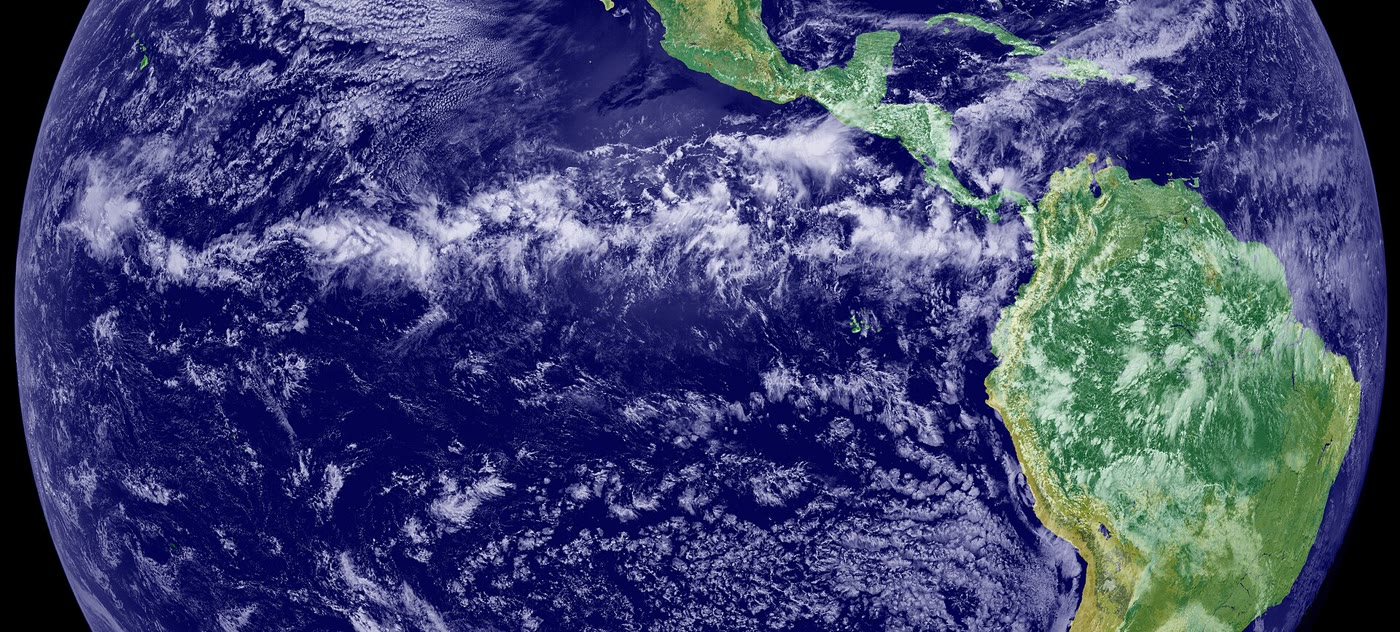
\includegraphics[width=0.8\linewidth]{images/book3/b1-itcz-goes.jpg}

{\small 东太平洋上的\omterm{def:b1:atmospheric-circulation:itcz}{热带辐合带}：一条明亮的云带
横跨赤道以北的海洋，右侧为中美洲与南美洲。
图像结合了 GOES-11 地球静止卫星的云层数据
与陆地覆盖的颜色。（NASA Earth Observatory，公有领域，
经维基共享资源提供。）}
\label{fig:b1:atmospheric-circulation:itcz-photo}
\end{omfigure}
% ledger: commons:itcz-goes

辐合的空气必然上升，上升的湿润空气会形成云：\omterm{def:b1:atmospheric-circulation:itcz}{热带辐合带}是全球降水最多的地带，
其位置可由纬向平均降水峰值所在的\omterm{def:b1:spherical-astronomy:geographic}{纬度}来标定。\omterm{def:b1:atmospheric-circulation:itcz}{热带辐合带}跟随太阳移动，
但有一定延迟。再分析资料显示，降水峰值在 2 月位于南纬 \ang{12.8}，
9 月移至北纬 \ang{10.9}；十二个月平均而言位于北纬 \ang{2.6}。
纬向平均掩盖了\omterm{def:b1:spherical-astronomy:geographic}{经度}间的巨大差异：照片中的东太平洋上，
云带位于赤道以北，
而纬向平均则将这些云带与其他随季节摆动得更远的云带
平均在一起。
% ledger: data:b3-ncep (computed in figdata/bachelor-1/general_circulation.py)

\begin{omfigure}
\begin{tikzpicture}
\begin{axis}[omrecord, width=0.7\linewidth, height=5.2cm, xmin=0.5, xmax=12.5, ymin=-16, ymax=16,
  xlabel={月份}, ylabel={纬度 (\unit{\degree})}, xtick={1,...,12},
  xticklabels={1,2,3,4,5,6,7,8,9,10,11,12}, ytick={-15,-10,...,15}]
% figdata/bachelor-1/general_circulation.py; ledger: data:b3-ncep
\addplot[black!40, domain=0.5:12.5] {0};
\addplot[omThm, line width=1.1pt, mark=*, mark size=1.6pt] table[x=month, y=lat] {figdata/out/bachelor-1-general_circulation-itcz.dat};
\end{axis}
\end{tikzpicture}

{\small 逐月的纬向平均降水极大值\omterm{def:b1:spherical-astronomy:geographic}{纬度}，
范围为南纬 \ang{20} 至北纬 \ang{20}：\omterm{def:b1:atmospheric-circulation:itcz}{热带辐合带}
在北半球夏季向北移动，在南半球夏季向南移动，比太阳
滞后两到三个月。
数据来自 NCEP-NCAR Reanalysis~1，取 1991--2020 年平均值，数据由 NOAA PSL 提供。}
\label{fig:b1:atmospheric-circulation:itcz}
\end{omfigure}
% ledger: data:b3-ncep

沿赤道本身，$f = 0$，空气沿气压梯度直接下沉，
于是在太平洋上方出现东西向的环流。

\begin{definition}[沃克环流]\label{def:b1:atmospheric-circulation:walker}
\emph{沃克环流}\index{沃克环流}是沿赤道太平洋的大气
东西向翻转环流圈：空气在西部温暖的海面上方上升，
绕过海洋大陆，在高空向东流动，在东太平洋下沉，
并在近地面随\omterm{def:b1:atmospheric-circulation:winds}{信风}向西返回。
\end{definition}
% ledger: climategov:walker

\begin{omfigure}
\begin{tikzpicture}[>={Stealth[length=2mm]}, font=\scriptsize]
  \fill[blue!12] (0,0) rectangle (11,0.45);
  \shade[left color=orange!45, right color=blue!12] (0,0) rectangle (6,0.45);
  \fill[brown!45] (-0.9,0) rectangle (0,0.6);
  \fill[brown!45] (11,0) rectangle (11.9,0.6);
  \node[anchor=north] at (-0.45,-0.05) {海洋};
  \node[anchor=north] at (-0.45,-0.35) {大陆};
  \node[anchor=north] at (11.45,-0.05) {南};
  \node[anchor=north] at (11.45,-0.35) {美洲};
  \node[anchor=north] at (5.5,-0.05) {赤道太平洋};
  \node at (1.6,0.22) {暖水};
  \foreach \x in {0.6,1.2,1.8} \fill[black!20] (\x,2.6) circle (0.45);
  \foreach \x in {0.9,1.5} \fill[black!25] (\x,3.0) circle (0.4);
  \draw[line width=1.2pt, omThm, ->] (9.5,0.8) -- (2.0,0.8);
  \draw[line width=1.2pt, omThm, ->] (1.2,1.0) -- (1.2,3.0);
  \draw[line width=1.2pt, omThm, ->] (2.0,3.3) -- (9.5,3.3);
  \draw[line width=1.2pt, omThm, ->] (10.3,3.0) -- (10.3,1.0);
  \node[anchor=south] at (5.75,0.85) {信风，自东向西};
  \node[anchor=south] at (5.75,3.35) {高空回流，自西向东};
  \node[anchor=west, align=left] at (1.6,1.8) {上升气流，\\大雨};
  \node[anchor=east, align=right] at (10.0,1.8) {下沉气流，\\干燥};
\end{tikzpicture}

{\small 沿赤道太平洋的\omterm{def:b1:atmospheric-circulation:walker}{沃克环流}（示意图，高度未按比例）：
西部暖水上空上升，高空向东流动，东部下沉，
近地面随\omterm{def:b1:atmospheric-circulation:winds}{信风}向西返回。}
\label{fig:b1:atmospheric-circulation:walker}
\end{omfigure}
% ledger: climategov:walker

\omterm{def:b1:atmospheric-circulation:walker}{沃克环流}并不稳定。当它减弱时，
海洋大陆上空的上升运动随之减弱，那里的空气甚至可能下沉；当它增强时，
西部的上升运动和降雨都会加强。这些起伏，即厄尔尼诺与拉尼娜，
以及季风的季节性反转，是本科二年级分册的内容。
自 1980 年以来的数十年间，IPCC 2021 年的评估认为，\omterm{def:b1:atmospheric-circulation:walker}{沃克环流}\emph{很可能}增强，
接近拉尼娜状态，并向西移动，
对变化幅度的把握程度为\emph{中等信度}。
% ledger: climategov:walker, ipcc:hadley-widening

\section{急流}\label{sec:b1:atmospheric-circulation:jets}

\begin{definition}[急流；副热带急流与极锋急流]\label{def:b1:atmospheric-circulation:jet}
\emph{急流}\index{急流}是狭窄的强风带，通常为
对流层高层的水平风，其位置逐日变化。\emph{副热带急流}\index{副热带急流}
在\omterm{def:b1:atmospheric-circulation:cells}{哈得来环流圈}的极向边缘附近由西向东吹，
通常位于\omterm{def:b1:spherical-astronomy:geographic}{纬度} \ang{20} 至 \ang{30} 之间，
高度为 \qtyrange{12}{14}{km}。\emph{极锋急流}\index{极锋急流}
在极地空气与副热带空气交界的上方由西向东吹，
位于约 \ang{50} 至 \ang{60} 之间；它是\omterm{def:b1:atmospheric-circulation:winds}{西风带}的快速核心，
既受中\omterm{def:b1:spherical-astronomy:geographic}{纬度}低压与\omterm{def:b1:atmospheric-circulation:cyclone}{反气旋}的引导，又引导着它们。
\end{definition}
% ledger: nws:jets, noaajs:jet

\omterm{def:b1:atmospheric-circulation:jet}{急流}通常出现在 \qty{9}{km} 附近，风速可超过
\qty{440}{km/h}，并在各半球的冬季最强，此时
热带与极地之间的温差最大。\omterm{def:b1:atmospheric-circulation:jet}{副热带急流}是
\cref{prop:b1:atmospheric-circulation:angular-momentum}所述的角动量风，
受涡旋调制；它位于\omterm{def:b1:atmospheric-circulation:cells}{哈得来环流圈}的边缘，冬季平均位置在 \ang{30} 附近。
\omterm{def:b1:atmospheric-circulation:jet}{极锋急流}随经过的低压南北摆动，
而绕纬圈平均会把它抹平：在北半球夏季的纬向平均中，
只在北纬 \ang{42.5} 附近残留一个 \qty{21.6}{m/s} 的弱极大值，
在南半球夏季则于南纬 \ang{47.5} 附近为 \qty{29.9}{m/s}。
风随高度增大的原因，即温度向极地递减处的热成风，
见本科三年级分册。
% ledger: noaajs:jet, nws:jets, data:b3-ncep-circ (computed in figdata/bachelor-1/general_circulation.py)

\section{练习}

\begin{exercise}[$\star$]\label{exo:b1:atmospheric-circulation:1}
取 $\Omega = \qty{7.292e-5}{rad.s^{-1}}$。(a)~计算下列\omterm{def:b1:spherical-astronomy:geographic}{纬度}处的\omterm{def:b1:atmospheric-circulation:coriolis-parameter}{科里奥利参数}：
北纬 \ang{0}、\ang{30}、\ang{45} 和 \ang{90}。(b)~计算
北纬 \ang{45} 处、风速为 \qty{10}{m/s} 的风所受的水平科里奥利加速度，并将其与 $g =
\qty{9.81}{m.s^{-2}}$ 比较。(c)~若风向北吹，
该加速度指向哪个方向？
% ledger: earth:Trot
\end{exercise}

\begin{exercise}[$\star$]\label{exo:b1:atmospheric-circulation:2}
海平面处，等压线间隔 \qty{4}{hPa}，相距 \qty{400}{km}，此处 $\rho =
\qty{1.225}{kg.m^{-3}}$。(a)~计算\omterm{def:b1:atmospheric-circulation:pgf}{气压梯度力}产生的
加速度。(b)~若无其他作用力，静止空气加速到 \qty{10}{m/s}
需要多长时间？(c)~将此加速度与北纬 \ang{45} 处风速为
\qty{10}{m/s} 的风的科里奥利加速度比较，并说明这意味着什么。
% ledger: ussa76:sea-level, earth:Trot
\end{exercise}

\begin{exercise}[$\star$]\label{exo:b1:atmospheric-circulation:3}
在北纬 \ang{40}，等压线间隔 \qty{4}{hPa}，相距 \qty{250}{km}；取 $\rho =
\qty{1.225}{kg.m^{-3}}$。(a)~计算\omterm{def:b1:atmospheric-circulation:geostrophic}{地转风}，分别以 \unit{m/s} 和节表示
（\qty{1}{kn} = \qty{0.5144}{m/s}）。(b)~低压位于南侧，
风从哪个方向吹来？(c)~描述预报员会绘制的风羽符号
（风杆与风羽）。
% ledger: ussa76:sea-level, earth:Trot
\end{exercise}

\begin{exercise}[$\star$]\label{exo:b1:atmospheric-circulation:4}
再分析资料的年平均值给出近地面的向东风速：
北纬 \ang{15} 处为 \qty{-3.5}{m/s}，南纬 \ang{15} 处为 \qty{-4.4}{m/s}，北纬 \ang{45} 处为 \qty{+1.9}{m/s}，
南纬 \ang{45} 处为 \qty{+6.5}{m/s}，海平面气压在北纬 \ang{15} 处为
\qty{1011.8}{hPa}，北纬 \ang{30} 处为 \qty{1016.8}{hPa}，
北纬 \ang{45} 处为 \qty{1015.8}{hPa}。(a)~说出四个\omterm{def:b1:spherical-astronomy:geographic}{纬度}各自所在的风带。
(b)~用环流圈近地面分支解释每种风的正负号。(c)~根据这些气压值，
北半球\omterm{def:b1:atmospheric-circulation:cells}{副热带高压}位于何处？
% ledger: data:b3-ncep-circ
\end{exercise}

\begin{exercise}[$\star\star$]\label{exo:b1:atmospheric-circulation:5}
气压梯度为每 \qty{500}{km} \qty{2}{hPa}，$\rho =
\qty{1.225}{kg.m^{-3}}$，在北纬 \ang{60}、\ang{50}、\ang{30}、\ang{20}、
\ang{10} 和 \ang{5} 处的情形。(a)~计算各\omterm{def:b1:spherical-astronomy:geographic}{纬度}的\omterm{def:b1:atmospheric-circulation:geostrophic}{地转风}。
(b)~在这样的梯度下，深热带的真实风速很少超过每秒几米。
解释\omterm{def:b1:atmospheric-circulation:geostrophic}{地转平衡}为何在赤道附近失效，
借助科里奥利力使风转向所需的时间 $1/f$ 来说明。
% ledger: ussa76:sea-level, earth:Trot
\end{exercise}

\begin{exercise}[$\star\star$]\label{exo:b1:atmospheric-circulation:6}
(a)~由\cref{prop:b1:atmospheric-circulation:angular-momentum}，计算
从赤道静止出发的空气环在 \ang{10}、\ang{15}、\ang{20} 和
\ang{30} 处的风速；取 $\Omega a_\oplus = \qty{464.6}{m/s}$。(b)~对于在
\ang{10}、\ang{15}、\ang{20} 和 \ang{30} 处静止出发的空气环，求其风速。(c)~\omterm{def:b1:atmospheric-circulation:cells}{哈得来环流圈}的上升支
分布于一段\omterm{def:b1:spherical-astronomy:geographic}{纬度}范围，而非恰好位于赤道，
这将如何改变预测的\omterm{def:b1:atmospheric-circulation:jet}{急流}？
% ledger: earth:Trot, earth:Rmean
\end{exercise}

\begin{exercise}[$\star\star$]\label{exo:b1:atmospheric-circulation:7}
(a)~位于北半球的一艘船测得风来自西南方。运用
布伊斯-巴洛特定律，低压中心位于何处？(b)~位于南半球的一艘船测得风来自西北方。
低压位于何处？(c)~靠近地面时，
风斜穿等压线吹向低压。这是否改变你对 (a) 的答案，
即通过使低压方向顺时针或逆时针偏转？
% ledger: skybrary:buys-ballot
\end{exercise}

\begin{exercise}[$\star\star$]\label{exo:b1:atmospheric-circulation:8}
(a)~计算赤道与北纬 \ang{30} 之间、
\qty{1000}{hPa} 与 \qty{100}{hPa} 两气压面之间的空气质量，取 $a_\oplus = \qty{6371}{km}$ 和
$g = \qty{9.81}{m.s^{-2}}$。(b)~在年平均情况下，再分析资料中的北半球
\omterm{def:b1:atmospheric-circulation:cells}{哈得来环流圈}的输送量为 \qty{8.7e10}{kg/s}。要使该质量
穿过此环流圈一次需要多长时间？(c)~对北半球冬季环流圈，问题相同，
其输送量为 \qty{21.4e10}{kg/s}。
% ledger: earth:Rmean, data:b3-ncep-circ
\end{exercise}

\begin{exercise}[$\star\star$]\label{exo:b1:atmospheric-circulation:9}
设\omterm{def:b1:atmospheric-circulation:cells}{副热带高压}之下空气以 \qty{1}{cm/s} 下沉，
且空气是不饱和的。(a)~一天内它下沉多远？(b)~若无其他作用，
空气一天升温多少（取\omterm{def:b1:fluid-envelopes-structure:lapse-rate}{干绝热递减率}为 \qty{9.8}{K/km}）？(c)~
空气并不会逐日如此升温。在
\cref{ch:b1:radiation-heat-transport}中，哪一过程平衡了升温？(d)~为何许多
大型炎热沙漠位于这些高压之下？
% ledger: nws:dalr
\end{exercise}

\begin{exercise}[$\star\star\star$]\label{exo:b1:atmospheric-circulation:10}
在北纬 \ang{50}，取 $f = \qty{1.117e-4}{s^{-1}}$，并设等压线为半径
$r = \qty{500}{km}$ 的圆形等压线（见\cref{rem:b1:atmospheric-circulation:gradient}）。(a)~围绕
\omterm{def:b1:atmospheric-circulation:geostrophic}{地转风}速为 \qty{15}{m/s} 的低压区，解 $V^2/r + fV =
f|\vec v_g|$ 求梯度风 $V$。(b)~围绕一高压，证明 $V^2/r - fV + f
|\vec v_g| = 0$ 仅当 $|\vec v_g| \leq fr/4$ 时有解，并计算该极限。
(c)~(b) 的结论对\omterm{def:b1:atmospheric-circulation:cyclone}{反气旋}中心附近等压线间距意味着什么，
与低压区相比如何？
\end{exercise}

\begin{exercise}[$\star\star\star$]\label{exo:b1:atmospheric-circulation:11}
(a)~证明对小的 $\varphi$（以弧度计），从赤道静止出发的空气环的风速
为 $u \approx \Omega a_\oplus\varphi^2$。(b)~将该近似与
\ang{10} 处的精确公式作比较，取 $\Omega a_\oplus = \qty{464.6}{m/s}$。(c)~再分析资料中
\qty{200}{hPa} 处的年平均风速峰值为 \qty{27.0}{m/s}，
约位于北纬 \ang{35}。该空气环在何\omterm{def:b1:spherical-astronomy:geographic}{纬度}可达此速度？(d)~
此结果说明角动量论证在多大程度上可以信赖？
% ledger: earth:Trot, earth:Rmean, data:b3-ncep-circ
\end{exercise}

\begin{exercise}[$\star\star\star$]\label{exo:b1:atmospheric-circulation:12}
再分析资料中纬向平均降水的峰值位于下列\omterm{def:b1:spherical-astronomy:geographic}{纬度}（按
一月至十二月）：\ang{-10.5}、\ang{-12.8}、\ang{-5.8}、\ang{-4.6}、\ang{5.5}、
\ang{7.3}、\ang{8.6}、\ang{10.4}、\ang{10.9}、\ang{9.1}、\ang{7.4}、\ang{6.2}
（负值表示南纬）。(a)~计算年平均值与极差。(b)~次太阳点\omterm{def:b1:spherical-astronomy:geographic}{纬度}在
六月和十二月达到极端。ITCZ 落后于它几个月，
以及气候系统中哪一部分能够储存热量而造成这种滞后？
(c)~设在某一大洋上，ITCZ 全年位于赤道以北。说明
纬向平均为何仍可跨越赤道。
% ledger: data:b3-ncep
\end{exercise}

\section{问题：读取中纬度天气图}

\begin{problem}[{周末问题——北纬 \ang{50} 附近一站点的风}]
\label{pb:b1:atmospheric-circulation:1}
% values: calc/ch28.py (invented map; jet from data:b3-ncep-circ)
北大西洋的一张天气图显示，在北纬 \ang{50} 处的站点 P 附近，
等压线东西\omterm{def:b1:geological-maps:attitude}{走向}，每隔 \qty{4}{hPa} 一条，
气压较低者位于北侧。P 位于 \qty{1004}{hPa} 与 \qty{1008}{hPa} 两条等压线之间，
二者在该处相距 \qty{250}{km}；其海平面气压为 \qty{1006}{hPa}，气温为
\qty{10}{\degreeCelsius}。该图为虚构，但其数值具有典型性。
取 $\Omega = 2\pi/(\qty{23.9345}{h})$，$a_\oplus = \qty{6371}{km}$，$R_d =
\qty{287.05}{J.kg^{-1}.K^{-1}}$，为干空气的气体常数，\qty{1}{kn} = \qty{0.514444}{m/s}。

\medskip
\noindent\textbf{第一部分——气压梯度与\omterm{def:b1:atmospheric-circulation:geostrophic}{地转风}。}
\begin{enumerate}
  \item 用理想气体定律计算 P 处空气的密度。
  \item 计算 P 处的水平气压梯度，单位为 \unit{Pa.m^{-1}}。
  \item 计算\omterm{def:b1:atmospheric-circulation:pgf}{气压梯度力}产生的加速度。
  \item 计算北纬 \ang{50} 处的 $\Omega$ 与\omterm{def:b1:atmospheric-circulation:coriolis-parameter}{科里奥利参数}。
  \item 计算 P 处的\omterm{def:b1:atmospheric-circulation:geostrophic}{地转风}速。
  \item 分别以节和 \unit{km/h} 表示该风速。
  \item 证明：仅靠\omterm{def:b1:atmospheric-circulation:pgf}{气压梯度力}使静止空气达到\omterm{def:b1:atmospheric-circulation:geostrophic}{地转风}速所需的时间，
        为 $1/f$，并计算该时间，以及
        科里奥利力使风转过一整圈所需的时间 $2\pi/f$。
\end{enumerate}

\medskip
\noindent\textbf{第二部分——方向与半球。}
\begin{enumerate}[resume]
  \item \omterm{def:b1:atmospheric-circulation:pgf}{气压梯度力}在 P 处指向哪个方向？\omterm{def:b1:atmospheric-circulation:geostrophic}{地转风}
        沿哪个方向吹，
        风从哪一\omterm{def:b1:spherical-astronomy:horizontal}{方位角}吹来？
  \item 用布伊斯-巴洛特定律检验你的答案。
  \item 描述 P 处所画的风羽：风杆的方向、
        羽毛的数目，以及羽毛所在的一侧。
  \item 设相同的等压线，低压位于北侧，出现在
        南纬 \ang{50}。风将从哪个方向吹来？
  \item 在相同的密度与气压梯度下，计算
        北纬 \ang{30} 与北纬 \ang{60} 处的\omterm{def:b1:atmospheric-circulation:geostrophic}{地转风}。
  \item 计算北纬 \ang{5} 处的\omterm{def:b1:atmospheric-circulation:geostrophic}{地转风}。该结果是否可信？请说明理由。
\end{enumerate}

\medskip
\noindent\textbf{第三部分——地面风。}P 处的风速计测得
风速为 \qty{9.0}{m/s} 的风，以 \ang{25} 的夹角穿越等压线，指向低压。
\begin{enumerate}[resume]
  \item 计算实测风速与\omterm{def:b1:atmospheric-circulation:geostrophic}{地转风}速之比，以及
        实测风沿等压线方向与垂直等压线方向的分量。
  \item 实测风从哪个\omterm{def:b1:spherical-astronomy:horizontal}{方位角}吹来？
  \item 在\cref{prop:b1:atmospheric-circulation:friction}的线性阻力模型中，
        求使模型给出实测偏角的时间常数 $\tau$，以及此时模型预测的风速，
        并与观测结果进行比较。
  \item 设半径为 \qty{500}{km} 的低压区周围，
        近地面最低一千米内的空气处处向内流动，其垂直等压线分量
        与第~14~题相同，密度与第~1~题相同，计算
        每秒进入该低压的空气质量。
  \item 这些空气必须从该层顶部流出。计算该处的平均上升速度，
        分别以 \unit{m/s} 和米每天表示。
  \item 取\omterm{def:b1:fluid-envelopes-structure:lapse-rate}{干绝热递减率} \qty{9.8}{K/km}，上升空气
        一天内降温多少？随之会出现什么天气？
        若改为\omterm{def:b1:atmospheric-circulation:cyclone}{反气旋}，情况又如何？
\end{enumerate}

\medskip
\noindent\textbf{第四部分——上方的\omterm{def:b1:atmospheric-circulation:jet}{急流}。}北半球冬季在 \qty{200}{hPa} 高度上的纬向平均风
在北纬 \ang{30} 附近达到峰值 \qty{42.3}{m/s}（再分析资料平均，
1991--2020）。
\begin{enumerate}[resume]
  \item 计算赤道与北纬 \ang{30} 处地面向东的速度。
  \item 一圈空气从赤道高空静止出发，并保持角动量
        守恒。计算其在北纬 \ang{20} 与北纬 \ang{30} 处的风速。
  \item 对从北纬 \ang{10} 静止出发的一圈空气，求其在北纬 \ang{30} 处的风速，问题同上。
  \item 第~21~题中的那一圈空气在北纬 \ang{30} 处的风速，
        是北纬 \ang{30} 处实测\omterm{def:b1:atmospheric-circulation:jet}{急流}的多少倍？请给出实际\omterm{def:b1:atmospheric-circulation:jet}{急流}较慢的两个原因。
  \item 计算实测\omterm{def:b1:atmospheric-circulation:jet}{急流}在北纬 \ang{30} 处单位质量的绝对角动量，
        与赤道静止空气单位质量绝对角动量之比。
        沿途损失了多大比例？
  \item P 处的\omterm{def:b1:atmospheric-circulation:geostrophic}{地转风}速为多少（以米每秒为单位），
        地面实测风与之相比如何？
\end{enumerate}
\end{problem}
